\section{Introduction}
Machine learning systems trained on sensitive user data can be vulnerable to privacy attacks~\citep{shokri2017membership,hayes2019logan}.
This issue is especially pressing for recent applications of large language models, as these models are capable of memorizing and reconstructing sensitive examples contained in 
the training data~\citep{DBLP:journals/corr/ZhangBHRV16, carlini2020extracting}.

As a result of these concerns, there has been a large interest in developing
methods that provide data privacy guarantees for large language models.
The standard paradigm for providing such a guarantee in machine learning is \textit{Differential Privacy} (DP)~\citep{dwork2006calibrating,dwork2014algorithmic}.
Unfortunately, DP learning has typically struggled to produce useful models when applied to large language models, resulting in models with either vacuous privacy guarantees \citep{dupuy2021efficient} or performance far below non-private baselines.
This is widely attributed to the fact that the core primitive of \textit{Differentially Private Stochastic Gradient Descent} (DP-SGD)~\citep{song2013stochastic,bassily2014differentially,abadi2016deep} injects noise that must scale with the number of parameters, resulting in large noise levels for large language models \citep{yu2021not}.

We tackle the problem of building performant DP language models for sentence classification and language generation tasks with merely tens to hundreds of thousands of examples.
We pursue this goal by re-examining the performance of the baseline DP optimization algorithm for fine-tuning large language models, and study how choices of hyperparameters, training objective, and pretrained models affect the performance given fixed privacy budgets. 
In contrast to the mainstream perception, \textbf{our empirical results demonstrate that large pretrained models with hundreds of millions of parameters can be effectively and efficiently fine-tuned to yield models with high performance under modest privacy leakage.}
For sentence classification, the performance of our fine-tuned models surpasses those obtained under heuristic privacy notions~\citep{huang2020texthide} which do not possess formal privacy guarantees.
For text generation, the performance of our models surpasses strong non-private baselines. 
Figure~\ref{fig:fig1} illustrates some of these results and the overall scaling behavior.
We summarize our contributions below.
\begin{itemize}[leftmargin=6mm]
    \setlength\itemsep{0.2mm}
    \item [(1)] We show that with appropriate hyperparameters and downstream task objectives, fine-tuning pretrained language models with DP-SGD/DP-Adam yields strong performance for a suite of NLP tasks at privacy levels $\epsilon \in \{3, 8 \}$. 
      Some of our fine-tuned models outperform strong non-private learning baselines and models obtained under heuristic privacy notions. 
    \item [(2)] Running DP-SGD can be memory-intensive due to clipping per-example gradients.
      We present \textit{ghost clipping}, a memory saving technique that makes fine-tuning large Transformers under DP memory efficient.
      Our technique generalizes the~\cite{goodfellow2015efficient} trick to handle sequential inputs, and
      can be combined with a layer-by-layer clipping procedure~\citep{lee2020scaling} to enable privately fitting large Transformers with almost the same memory cost as non-private training---at the cost of one additional backward pass per processed batch.
    \item [(3)] We show that the dimensionality of gradient updates does not explain private fine-tuning performance.
      While there exist dimension-dependent lower bounds for private (convex) optimization~\citep{bassily2014differentially}, we find that larger pretrained models lead to better private fine-tuning results. Moreover, parameter-efficient adaptation methods that reduce the dimensionality of updates do not  necessarily outperform a baseline method that fine-tunes all model parameters.
\end{itemize}
Our empirical studies indicate that directly fine-tuning pretrained models with DP optimization results in performant DP language models under modest privacy budgets.
This enables building practical private NLP models for a range of common tasks where privacy could be at stake.

\begin{figure}[t]
\begin{center}
\begin{minipage}[t]{0.48\linewidth}
\centering
{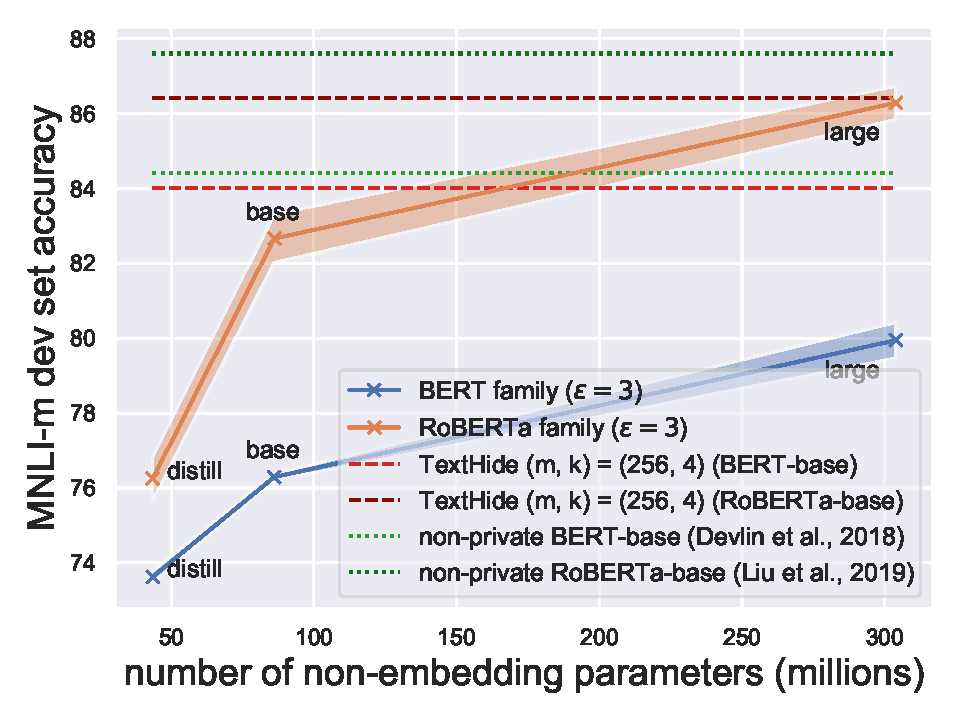
\includegraphics[width=0.98\textwidth]{figs/figure1_classification_v2.pdf}}
(a) Sentence classification \\MNLI-matched~\citep{williams2018multi}
\end{minipage}
\begin{minipage}[t]{0.48\linewidth}
\centering
{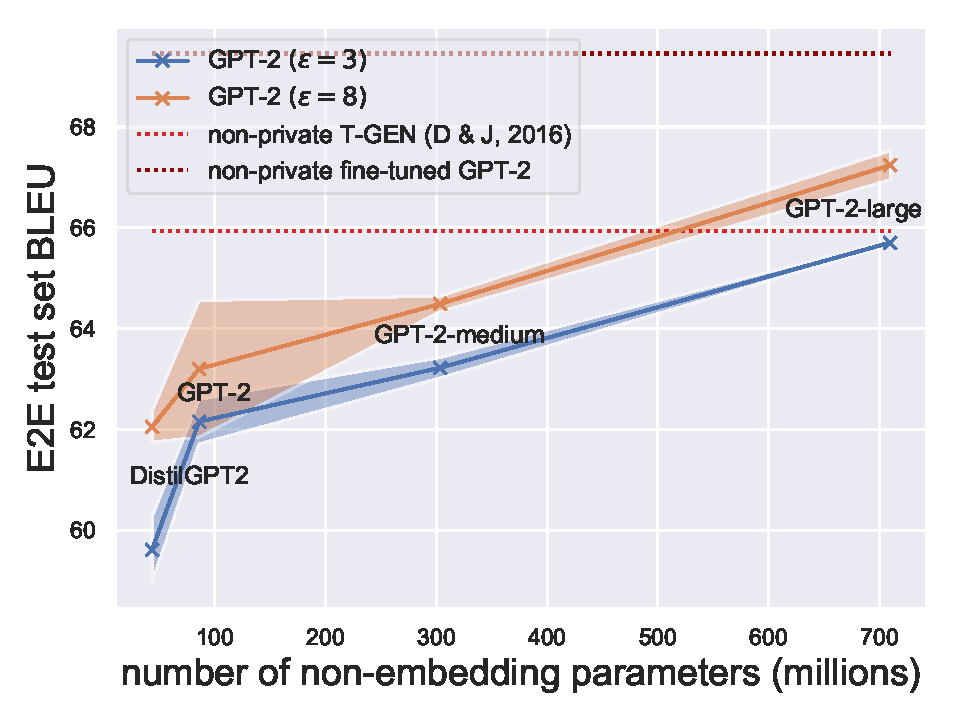
\includegraphics[width=0.98\textwidth]{figs/figure1_generation.pdf}}
(b) Natural language generation \\E2E~\citep{novikova2017e2e}
\end{minipage}
\end{center}
\caption{A summary of a few of our findings:
(1) Pretrained models fine-tuned with DP-Adam has strong performance. 
(2) Fine-tuning larger models produces better results. 
(3) Fine-tuned RoBERTa-large under DP at $\epsilon=3$ outperforms TextHide (the extension of InstaHide~\citep{huang2020instahide} for text classification) with BERT-base. 
Non-private generation baseline numbers are based on those reported by~\cite{wiseman2018learning}. 
}
\label{fig:fig1}
\end{figure}
